\documentclass[a4paper,11pt]{article}

\usepackage[portuguese]{babel}
\usepackage[utf8]{inputenc}
\usepackage[charter]{mathdesign} % charter or utopia?
\usepackage{multirow}
\usepackage[pdftex]{hyperref}
\usepackage{indentfirst}
\usepackage{xspace}
\usepackage[cm]{fullpage}
\usepackage{color, colortbl}
\usepackage{graphicx}
\usepackage{multirow}
\usepackage{fancyhdr}
\usepackage{tabu}
\usepackage{todonotes}
\usepackage[acronym,nowarn]{glossaries}
\newacronym{ASYNC}{ASYNC}{\textit{MPPA Asynchronous Communication}}
\newcommand{\async}{\gls{ASYNC}\xspace}

\newacronym{MPI}{MPI}{\textit{Message Passing Interface}}
\newcommand{\mpi}{\gls{MPI}\xspace}

\newacronym{openMP}{OpenMP}{\textit{Open Multi-Processing}}
    \newcommand{\openMP}{\gls{openMP}\xspace}

\newacronym{api}{API}{\textit{Application Programming Interface}}
    \newcommand{\api}{\gls{api}\xspace}
    \newcommand{\apis}{\glspl{api}\xspace}
    
\newacronym{hpc}{HPC}{computação de alto desempenho}
	\newcommand{\hpc}{\gls{hpc}\xspace}
	
\newacronym{cpu}{CPU}{\textit{Central Processing Unit}}
    \newcommand{\cpu}{\gls{cpu}\xspace}

    \newacronym{cpus}{CPUs}{\textit{Central Processing Units}}
    \newcommand{\cpus}{\gls{cpus}\xspace}

\newacronym{flops}{Flops}{\textit{Floating-point Operations per Second}}
    \newcommand{\flops}{\gls{flops}\xspace}

\newacronym{cnoc}{C-NoC}{\textit{Control NoC}}
    \newcommand{\cnoc}{\gls{cnoc}\xspace}

\newacronym{dnoc}{D-NoC}{\textit{Data NoC}}
    \newcommand{\dnoc}{\gls{dnoc}\xspace}

\newacronym{mpsoc}{MPSoC}{\textit{Multiprocessor System-on-Chip}}
    \newcommand{\mpsoc}{\gls{mpsoc}\xspace}

\newacronym{noc}{NoC}{\textit{Network-on-Chip}}
    \newcommand{\noc}{\gls{noc}\xspace}
    \newcommand{\nocs}{\glspl{noc}\xspace}

\newacronym{pe}{PE}{\textit{Processing Element}}
    \newcommand{\pe}{\gls{pe}\xspace}
    \newcommand{\pes}{\glspl{pe}\xspace}

\newacronym{rm}{RM}{\textit{Resource Manager}}
    \newcommand{\rman}{\gls{rm}\xspace}
    \newcommand{\rmans}{\glspl{rm}\xspace}

\newacronym{smp}{SMP}{\textit{Symmetric Multiprocessing}}
    \newcommand{\smp}{\gls{smp}\xspace}

\newacronym{spmd}{SPMD}{\textit{Single Program, Multiple Data}}
    \newcommand{\spmd}{\gls{spmd}\xspace}

    \newacronym{simd}{SIMD}{\textit{Single Instruction, Multiple Data}}
    \newcommand{\simd}{\gls{simd}\xspace}

\newacronym{vliw}{VLIW}{\textit{Very Long Instruction Word}}
    \newcommand{\vliw}{\gls{vliw}\xspace}

\newacronym{gpu}{GPU}{\textit{Graphics Processing Unit}}
    \newcommand{\gpu}{\gls{gpu}\xspace}
    \newcommand{\gpus}{\glspl{gpu}\xspace}

\newacronym{rapl}{RAPL}{\textit{Running Average Power Limit}}
    \newcommand{\rapl}{\gls{rapl}\xspace}

\newacronym{lpddr}{LPDDR3}{\textit{Low Power Double Data Rate 3}}
    \newcommand{\lpddr}{\gls{lpddr}\xspace}

\newacronym{io}{E/S}{Entrada e Saída}
    \newcommand{\io}{\gls{io}\xspace}
   
\newacronym{cc}{CC}{\textit{cluster} de computação}
	\newcommand{\cc}{\gls{cc}\xspace}

\newacronym{ccs}{CCs}{\textit{clusters} de computação}
	\newcommand{\ccs}{\gls{ccs}\xspace}

\newacronym{ipc}{IPC}{\textit{Inter-Process Communication}}
   \newcommand{\ipc}{\gls{ipc}\xspace}

\newacronym{numa}{NUMA}{\textit{Non-Uniform Memory Access}}
	\newcommand{\numa}{\gls{numa}\xspace}

\newacronym{ccnuma}{CC-NUMA}{\textit{Cache-Coherent Non-Uniform Memory Access}}
\newcommand{\ccnuma}{\gls{ccnuma}\xspace}

\newacronym{ncnuma}{NC-NUMA}{\textit{No Cache Non-Uniform Memory Access}}
\newcommand{\ncnuma}{\gls{ncnuma}\xspace}

\newacronym{soc}{SoC}{\textit{System-on-Chip}}
\newcommand{\soc}{\gls{soc}\xspace}

\newacronym{cmp}{CMP}{\textit{Chip Multiprocessor}}
\newcommand{\cmp}{\gls{cmp}\xspace}

\newacronym{cmps}{CMPs}{\textit{Chip Multiprocessors}}
\newcommand{\cmps}{\gls{cmps}\xspace}


\newacronym{uma}{UMA}{\textit{Uniform Memory Access}}
    \newcommand{\uma}{\gls{uma}\xspace}

\newacronym{ram}{RAM}{\textit{Random-Access Memory}}
    \newcommand{\ram}{\gls{ram}\xspace}

\newacronym{pc}{PC}{\textit{Personal Computer}}
    \newcommand{\pc}{\gls{pc}\xspace}

\newacronym{opengl}{OpenGL}{\textit{Open Graphics Library}}
    \newcommand{\opengl}{\gls{opengl}\xspace}

\newacronym{cow}{COW}{\textit{Clusters of Workstations}}
    \newcommand{\cow}{\gls{cow}\xspace}


\newacronym{now}{NOW}{\textit{Network of Workstations}}
    \newcommand{\now}{\gls{now}\xspace}

    \newacronym{so}{SO}{\textit{Sistema Operacional}}
    \newcommand{\so}{\gls{so}\xspace}

    \newacronym{e/s}{E/S}{\textit{Entrada e Saída}}
    \newcommand{\es}{\gls{e/s}\xspace}

%    \newacronym{kb}{KB}{\textit{Kilobyte}}
%    \newcommand{\kb}{\gls{kb}\xspace}
%
%    \newacronym{mb}{MB}{\textit{Megabyte}}
%    \newcommand{\mb}{\gls{mb}\xspace}
%    
%    \newacronym{gb}{GB}{\textit{Gigabyte}}
%    \newcommand{\gb}{\gls{gb}\xspace}

    \newacronym{posix}{POSIX}{\textit{Portable Operating System Interface}}
    \newcommand{\posix}{\gls{posix}\xspace}


\makeglossaries
\usepackage{subfigure}

\newcommand{\etal}{\textit{et al}.\xspace}
\newcommand{\eg}{\textit{e.g}.,\xspace}
\newcommand{\ie}{\textit{i.e}.,\xspace}
\newcommand{\pskel}{PSkel\xspace}
\newcommand{\pskelmppa}{PSkel-MPPA\xspace}
\newcommand{\mppa}{MPPA-256\xspace}
\newcommand{\fw}{\textit{framework}\xspace}
\newcommand{\capb}{CAP Bench\xspace}
\newcommand{\epiphany}{Adapteva Epiphany\xspace}
\newcommand{\manycore}{\textit{manycore}\xspace}
\newcommand{\manycores}{\textit{manycores}\xspace}
\newcommand{\bench}{\textit{benchmark}\xspace}

\fancypagestyle{plain}{%
	\renewcommand{\headrulewidth}{0pt}%
	\fancyhf{}%
	\fancyhead[C]{
		\begin{tabular*}{1.012\textwidth}{l@{\extracolsep{\fill} }cr}
			\multirow{2}{*}{\hspace{-0.3cm}
\includegraphics[height=2cm, width=!]{./figs/ufsc.jpg}} & \hspace{0.8cm}Universidade Federal de Santa Catarina (UFSC) & \multirow{2}{*}{
\includegraphics[height=2cm, width=!]{./figs/ine.pdf}} \\
			& \hspace{0.8cm}Departamento de Informática e Estatística (INE) & \\
		\end{tabular*}
	}%
}

\title{\hspace{-0.6cm}\textbf{Relatório Final - PIBIC 2018/2019}\\[0.2cm] \hspace{-0.6cm}\textbf{Projeto:} Otimização do Benchmark \capb para o Processador Manycore de Baixo Consumo Energético \mppa}
\author{\hspace{-0.6cm}\textbf{Bolsista:} David Grunheidt Vilela Ordine\\\hspace{-0.6cm}\textbf{Orientador:} Prof. Dr. Márcio Castro\\ \hspace{-0.6cm}\small{\emph{Laboratório de Pesquisa em Sistemas Distribuídos (LaPeSD), INE/UFSC}}}
\date{\hspace{-0.6cm}\small{Florianópolis, \today}}
\begin{document}
\pagenumbering{gobble}%

\maketitle

\begin{abstract}
Similar ao que aconteceu com os processadores \textit{single-core}, ao longo de sua evolução, as tecnologias voltadas para \hpc depararam-se com uma barreia de potencia, a qual torna desvantajoso o \textit{trade-off} entre gasto energético e ganho em desempenho. Processadores \manycore de baixo consumo energético surgiram como uma possível solução para o problema, como o \mppa e o \epiphany. Devido a questões arquiteturais, como uma memória distribuída e limitada no \textit{chip}, a implementação de aplicações que beneficiam-se totalmente do \textit{hardware} mostra-se desafiadora. Neste projeto foram propostas otimizações para diversas aplicações do \capb: um \textit{benchmark} desenvolvido para avaliar o desempenho e o consumo de energia do \mppa. Os resultados mostram que as versões otimizadas das aplicações possuem um melhor desempenho que as versões anteriores. Isso se deve principalmente à otimização de partes da computação e pelo uso de uma nova biblioteca de comunicação assíncrona. \\

\noindent\textbf{Palavras-chave}: \textit{manycores}, MPPA-256, comunicação assíncrona.
\end{abstract}

\tableofcontents

\newpage

\section{Introdução}


Para que os supercomputadores atuais consigam alcançar de forma definitiva a computação em \textit{exaescale}, é necessário que haja, de forma coesa, alto desempenho e consumo energético viável. Porém, assim como ocorreu com os avanços nas tecnologias de processadores \textit{single-core}, os quais, nas ultimas três décadas, permitiram aumento no desempenho de um processador a uma taxa anual de 40\% a 50\%  \cite{Larus:2008:TM:1364782.1364800}, a dissipação de calor nos supercomputadores que utilizam processadores do tipo \textit{multicore} chegou a um ponto que não mais permitiu a escalabilidade proporcional das variáveis citadas acima.
 
Seguindo os conceitos de \textit{Green Computing}, estudos foram realizados a fim de encontrar um \textit{trade-off} positivo entre desempenho e gasto energético, centrado na redução do consumo de energia. O grande interesse da comunidade científica de \hpc acerca deste tema foi um dos responsáveis por alavancar a produção dos \manycores de baixa potência, tais quais, o \mppa \cite{MPPA-2:2013}, o SW26010, utilizado no supercomputador \textit{Sunway TaihuLight} \cite{sunway:2016} e o \epiphany  \cite{Olofsson2014}.

Com propósito de validar as supostas qualidades do \mppa e prover meios de comparação com outros processadores do estado da arte, \textit{Souza} \etal implementaram o \capb \cite{Castro-Souza-CCPE:2016}, \textit{benchmark} que avalia ambos desempenho e gasto energético do processador, levando em conta diversos cenários. Em sua versão inicial, utilizava uma \api de comunicação síncrona entre processos, denominada \ipc \cite{MPPA-2:2013}. Esta antiga \api possui algumas deficiências, como baixo nível de abstração e realização de sincronizações implícitas, levando a queda de desempenho.

Neste trabalho, a fim de implementar a otimização proposta, realizou-se o porte do \capb com a nova \api de comunicação assíncrona entre processos da Kalray, a \async \cite{Hascoet2017}. Esta \api possui nível de abstração superior a \ipc, além de diferir na implementação quanto ao modelo de lógica de memória. Assim, ela simplifica a elaboração de aplicações para o \mppa, além de ganhar em desempenho e reduzir o custo energético, devido a sua característica assíncrona.

\subsection{Objetivos}

O objetivo desta pesquisa de iniciação científica é propor e implementar a otimização do \bench \capb para o processador \manycore de baixo consumo energético \mppa. Os objetivos específicos deste projeto de pesquisa estão elencados abaixo:

\begin{enumerate}
	\setlength\itemsep{0em}
	\item Investigar a viabilidade do uso do \mppa para a computação científica de alto desempenho;
	\item Estudar as \apis de comunicação existentes para o \mppa.
	\item Implementar um conjunto de aplicações paralelas para o \mppa (\bench) utilizando-se da \api \async;
	\item Avaliar os custos e benefícios do \mppa em relação ao desempenho e ao consumo de energia, assim como sua utilidade para a Computação Sustentável (\textit{Green Computing});
	\item Difundir a pesquisa e os seus resultados através de produção científica de qualidade, em periódicos e eventos relevantes na área de Processamento Paralelo e Distribuído.
\end{enumerate}

Nas seções seguintes são apresentados o desenvolvimento e os resultados produzidos, de acordo com o cronograma e as atividades propostas deste projeto de pesquisa.

\section{Revisão Bibliográfica}

Esta seção apresenta a revisão bibliográfica sobre o processador \manycore \mppa, o \textit{benchmark} \capb e a \api utilizada para realizar a otimização proposta. Por fim, são apresentados alguns trabalhos relacionados.

\subsection{MPPA-256}
\label{subsec:mppa}

O \mppa é um processador voltado ao baixo consumo energético, o qual, desenvolvido pela empresa francesa Kalray, reflete o estado da arte dos processadores \manycore. A Figura \ref{fig:mppaOverview} mostra uma visão geral da arquitetura do processador, possuindo este 16 \ccs e 4 \textit{clusters} de \io. 	Os \textit{clusters} de \io realizam comunicações com dispositivos externos, tais quais, no caso da maquina utilizada nesta pesquisa, memórias \lpddr de 2GB. Já os \ccs possuem as seguintes características:
\begin{itemize}
	\item 16 núcleos de processamento, chamados de \pes, que executam, com frequência de 400 MHz, threads de usuário em modo ininterrupto e não preemptivo. Estes núcleos também possuem duas memórias \textit{cache}, uma para dados e outra para instruções. Ambas são associativas 2-\textit{way} privadas	e possuem 32kB \cite{Podesta2018}.
	\item Gerenciador de recursos para gerenciar as comunicações de um determinado \textit{cluster} e executar o sistema operacional.
	\item Memória compartilhada de 2MB, possibilitando, entre núcleos de um mesmo \textit{cluster}, alta largura de banda e alta taxa de transferência.
	\item Dois controladores, para dados e controle, da Rede-em-Chip (\noc) que conecta os \textit{clusters}.
\end{itemize}

\begin{figure}[t]
\centering
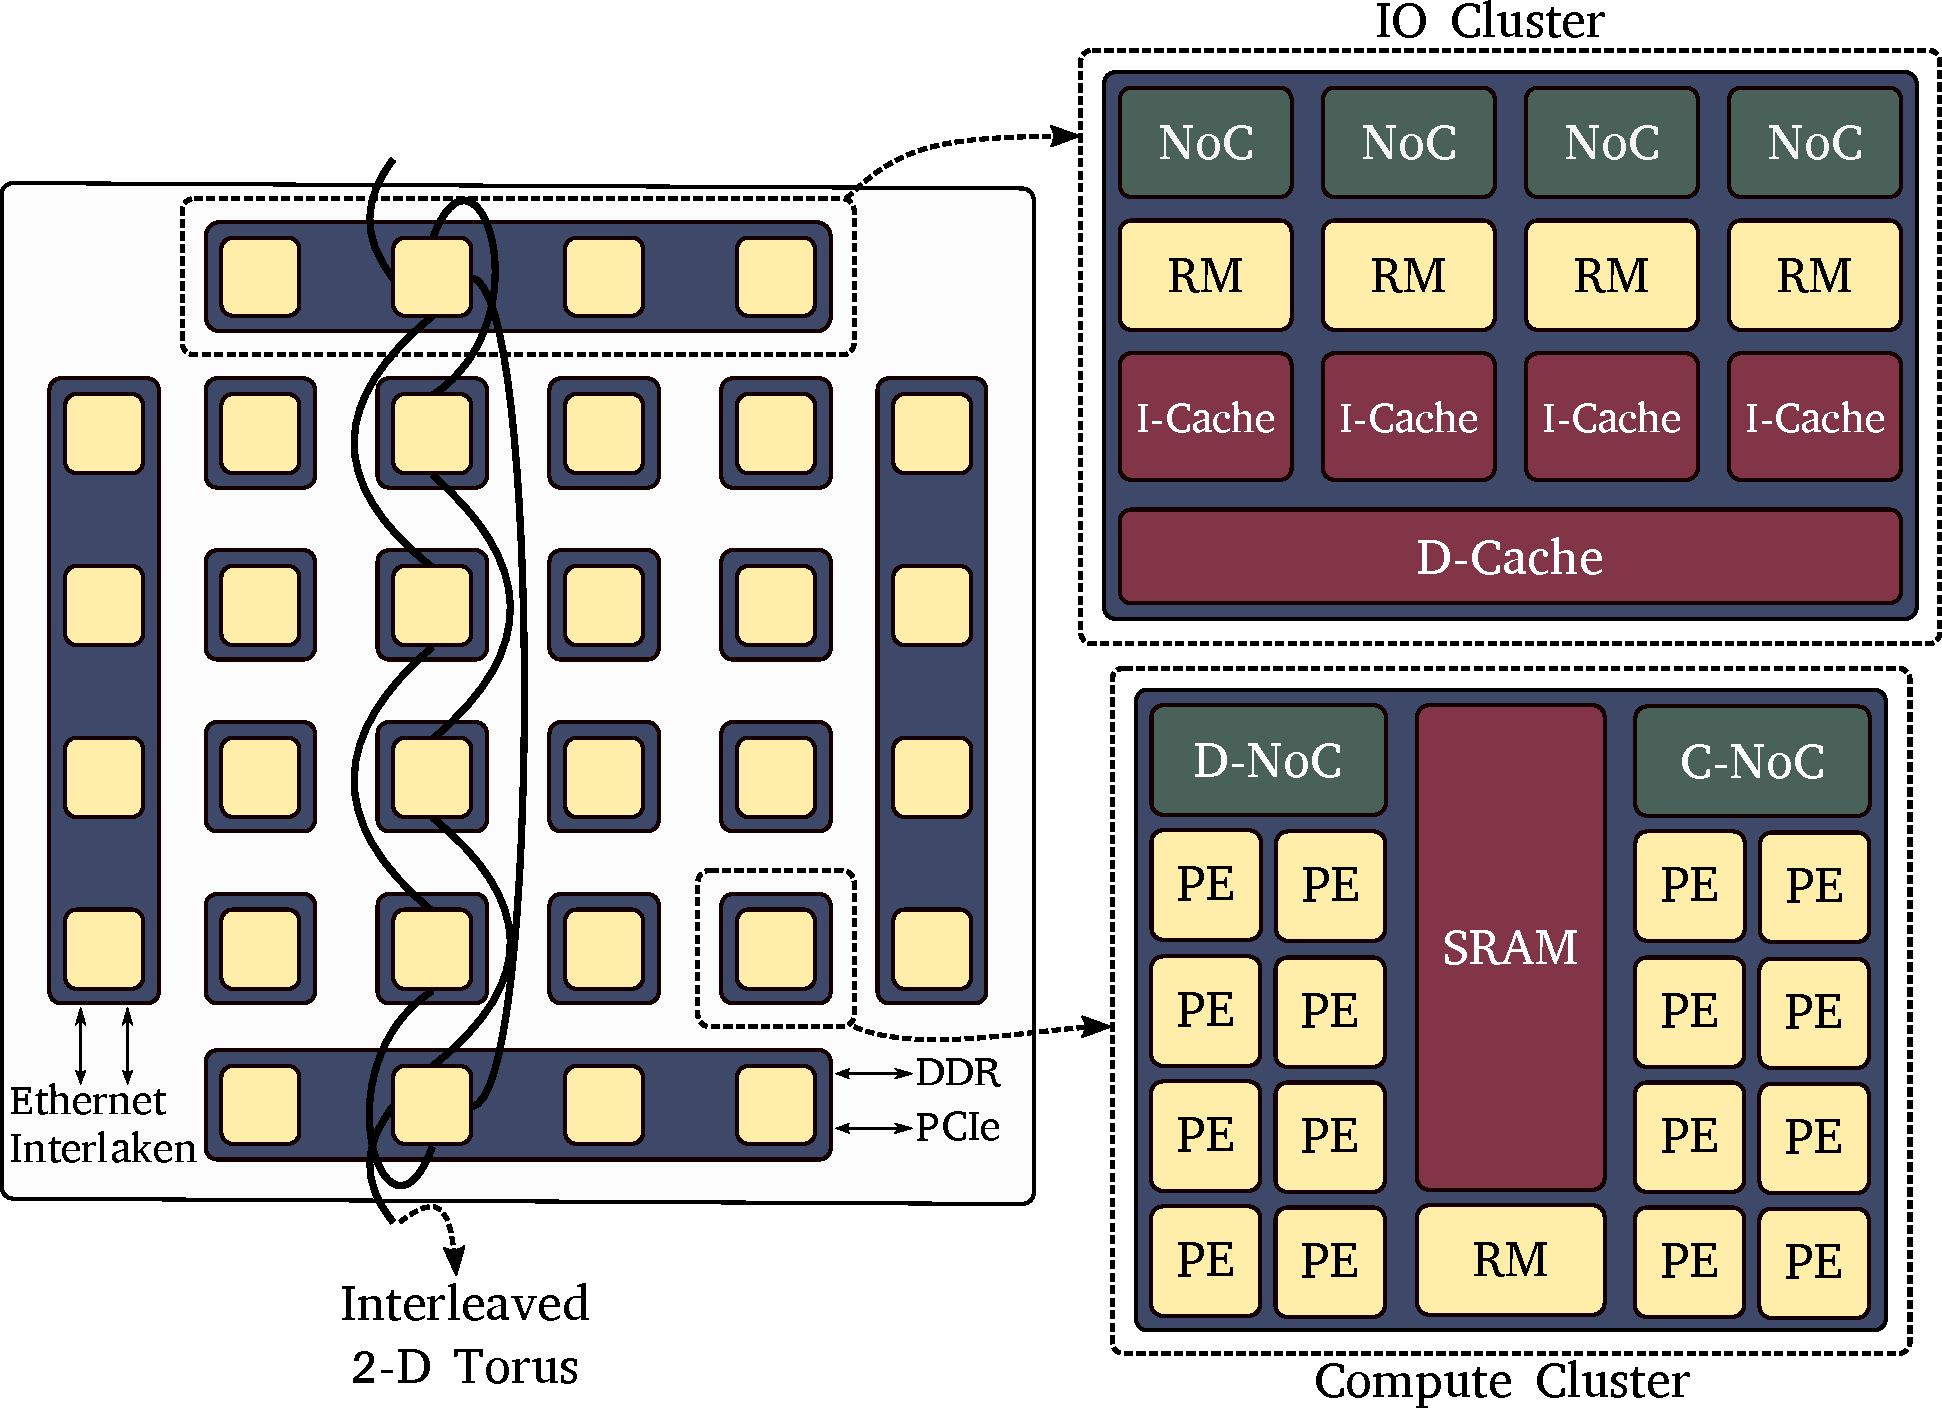
\includegraphics[width=9cm, keepaspectratio]{figs/mppa-overview.pdf}
\caption{Visão arquitetural simplificada do \mppa \cite{Penna2018}.}\par
\label{fig:mppaOverview}
\end{figure}

É importante salientar que ambos \ccs e \textit{clusters} de \io não podem acessar diretamente os dados armazenados na memória interna de um outro \textit{cluster} que não ele mesmo. Logo, o processador possui um modelo de memória distribuído \cite{Castro-Souza-CCPE:2016, Podesta2018}. Esta característica, comum a alguns processadores \manycore, é fator desafiador para implementação de aplicações paralelas otimizadas no \mppa \cite{Castro-IA3-JPDC:2014}. Neste trabalho, \textit{clusters} de \io serão também chamados de \textit{master} e \ccs serão também chamados de \textit{slaves}.

\subsection{\capb}
\label{subsec:capb}

O \capb é um \textit{benchmark} formado por 7 aplicações implementadas em C, diferindo na tecnologia de paralelismo utilizada dependendo da arquitetura alvo a ser testada. Atualmente, o \textit{benchmark} opera sobre arquiteturas x86, utilizando OpenMP e futuramente POSIX Threads. Também opera sobre o gem5 e o \mppa. O módulo voltado ao \mppa foi construído para testar todos os cenários de computação que este possa se deparar. Logo, as aplicações abrangem diversos problemas em diversos domínios, como grafos, ordenação e computação gráfica. Constituem o \capb os seguintes kernels: \textbf{(i)} Features from Accelerated Segment Test; \textbf{(ii)} Friendly Numbers; \textbf{(iii)} Gaussian Filter; \textbf{(iv)} Integer Sort; \textbf{(v)} K-Means; \textbf{(vi)} LU Factorization; e \textbf{(vii)} Traveling-Salesman Problem.

Originalmente, as aplicações voltadas ao \mppa foram desenvolvidas explorando a \api \ipc, da Kalray. Esta \api, baseada no padrão POSIX \ipc, lida com comunicações entre \ccs, e entre \ccs e \textit{clusters} de \io. Ao usar a \ipc, é preciso lidar com paralelismo explícito, onde o programador implementa o comportamento do paralelismo e cada unidade de trabalho é independente em termos de dados e computação \cite{Castro-Souza-CCPE:2016}


\subsection{Comunicação Assíncrona no \mppa}
\label{subsec:async}

Recentemente, a Kalray disponibilizou uma nova \api para comunicação assíncrona e unilateral entre os \textit{clusters} do \mppa, a \async. Esta nova \api abstrai o modelo de memória distribuído do \mppa e simula um contexto de memória compartilhada. Desta maneia, é possível, em um determinado \textit{cluster}, realizar operações assíncronas diretamente sobre os espaços de memória de outros \textit{clusters}. Para isso, a \api conta com diversas funcionalidades.

Em primeiro lugar, é preciso definir um segmento sobre uma porção de memória contígua de um \textit{cluster}. Outros \textit{clusters} podem então clonar este segmento, utilizando o \textit{id} próprio e único deste, o qual foi definido na sua criação. Após a clonagem, operações do tipo \texttt{put} e \texttt{get} podem ser realizadas sobre aquele segmento. A operação \texttt{get} copia um intervalo de dados, dentro do segmento, para dentro da memória local de um \textit{cluster}. Já a operação \texttt{put} envia um dado da memória local do \textit{cluster} para um intervalo de memória contido no segmento. Também existem inúmeras operações variantes das \texttt{put}/\texttt{get}, por exemplo, funções que trabalham com intervalos espaçados dentro de um segmento, intervalos de blocos 2D e até 3D, entre outras.

\begin{figure}[h]
\centering
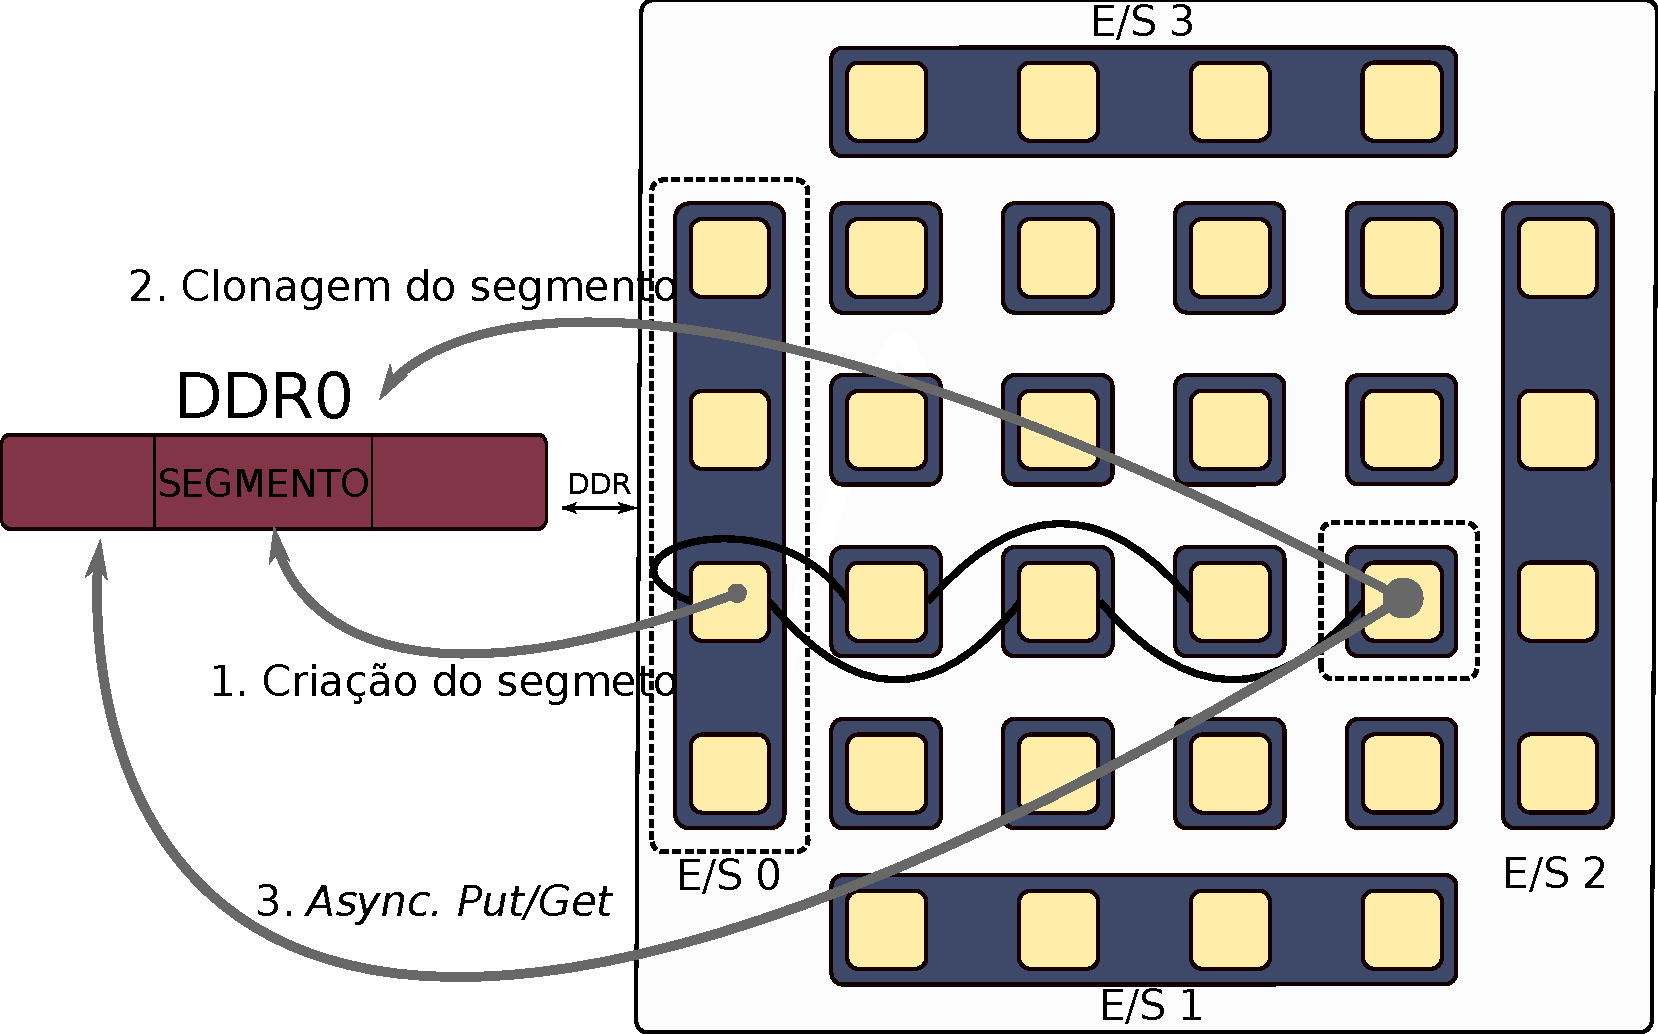
\includegraphics[width=9cm, keepaspectratio]{figs/putget.pdf}
\caption{Etapas da utilização da \api \async.}\par
\label{fig:asyncOverview}
\end{figure}

\todo[inline]{A Figura~\ref{fig:asyncOverview} mostra um exemplo de ...}

\subsection{Trabalhos Correlatos}

\section{Proposta e Implementação de Otimização no \capb}
\label{sec:capbMPPA}

Para a realização da otimização proposta, foi implementado, em todas as aplicações, uma nova lógica de comunicação entre \textit{clusters} de \io e \ccs, e entre \ccs, onde o uso da \async substituiu por completo o uso da antiga \ipc. Como a nova \api simula um modelo de memória compartilhada em suas operações, trabalhar com ela torna a tarefa de otimização consideravelmente mais fácil. Também são abrangidos, nesta nova lógica, diversas modificações sobre em qual tipo de \textit{cluster} é computado determinada operação de um \textit{kernel}, com objetivo de usufruir do poder de processamento dos \ccs, quando necessário, ou da memória local dos \textit{clusters} de \io, onde inicializa-se o dado a ser trabalhado. Todas as alterações serão mostradas detalhadamente, para cada \textit{kernel}, nesta seção. Uma descrição detalhada de cada um dos \textit{kernels} do \capb pode ser encontrada em \cite{Castro-Souza-CCPE:2016}.

\subsection{Alterações no Friendly Numbers}

Primeiramente, foi alterado a implementação da função que calculava a soma de todos os divisores de um certo inteiro. Em sua versão antiga, esta função realizava a busca dos divisores no intervalo entre 2 e aquele inteiro. Já na otimizada, a busca é feita entre 2 e a metade deste inteiro, pois, acima da metade, só existe ele como divisor de si mesmo. Quanto a utilização da \async, foi criado um segmento sobre o \textit{array} de itens a serem passados dos \textit{clusters} de \io para os \ccs, onde cada \cc possui um intervalo de \textit{offsets} no qual pode realizar operações sobre este segmento. Este intervalo é definido, em tempo de execução, no processo mestre no \textit{cluster} de \io, o qual repassa estas informações aos \textit{slaves} no momento que os inicializa.

\subsection{Alterações no LU Factorization}

Funções que setavam um novo pivô sobre a linha da matriz sendo iterada em algum \cc , realizando buscas por toda matriz e subsequentes trocas de linhas e colunas, foram removidas, pois, para calcular a fatoração LU não são permitidas tais operações, já que, ao realizá-las, é feito a decomposição PLU da matriz original, onde P é uma matriz de permutação. Além disso, a matriz L resultante não mais seria triangular inferior. Assim, sem as computações citadas acima, já é de se esperar ganho em desempenho enorme. Erros relacionados a passagem de tarefas dos \textit{clusters} de \io para os \ccs também foram corrigidos, pois, na versão antiga, os blocos dentro da matriz eram passados aos \textit{slaves} desalinhados, gerando descontinuidade na informação e resultado final errôneo. Para tirar proveito da \async neste \textit{kernel}, foi criado um segmento sobre a matriz original, representada por um \textit{array} unidimensional. Porém, diferentemente do FN, ao iniciar os \textit{slaves}, só é informado a eles o tamanho da matriz a ser decomposta. Auxiliar ao segmento da matriz, foi criado um segmento para conter os \textit{offsets} que serão utilizados pelos \ccs, no segmento da matriz, em uma certa iteração. É sobre este segmento que, em diversos momentos, cada \cc retira a informação sobre qual intervalo de \textit{offsets}, no segmento da matriz, ele deve pegar o dado. Não foi preciso informar aos \textit{slaves}, em sua inicialização, qual é seu \textit{offset} no segmento de \textit{offsets} visto que seu próprio \textit{id} pode ser utilizado para isto.

\subsection{Alterações no K-Means}

Neste \textit{kernel}, diversas simplificações foram feitas. Primeiramente, para criar somente um segmento sobre a porção de dados a ser apurada e utilizar a \async de modo otimizado, foi necessário transformar o modelo de dados da aplicação. Antigamente, os pontos eram definidos como \textit{structs}, chamadas de vetores, contendo o tamanho (dimensão do vetor) e um ponteiro para os elementos (coordenadas do vetor). Porém, como todos os vetores possuem o mesmo tamanho, já que a dimensão é tratada globalmente, foi possível otimizar este modelo de dados, setando todos os pontos em um único \textit{array} unidimensional, o qual criou-se um segmento sobre. Vale salientar que a criação deste \textit{array} toma muito menos instruções do que a criação do \textit{array} de \textit{arrays} anterior. Desta maneira, em um cenário com $\mathnormal{P}$ pontos, todos com dimensão $\mathnormal{X}$, cada ponto ocupa $\mathnormal{X}$ posições do \textit{array} e o tamanho total deste é de $\mathnormal{X}$ $\times$ $\mathnormal{P}$ posições. Para recalcular os \textit{centroids}, na antiga versão, toda a computação de cálculo da distância euclidiana média era feita nos \ccs. Isto requeria que os \ccs enviassem a informação sobre suas populações parciais para os \textit{clusters} de \io, os quais passariam de volta a soma destes dados a todos os \ccs. Já na nova, nos \ccs é realizado somente a primeira etapa deste cálculo, sendo esta a soma dos seus vetores parciais. Para calcular a média, a população total é necessária, a qual está facilmente disponível nos \textit{clusters} de \io após determinada iteração. Assim, menos comunicações são feitas entre \textit{clusters}, \todo{na versão antiga não tinha put/get}{mais especificamente, 3 operações \textit{GET} e 3 \textit{PUT}, ao contrario das 5 operações \textit{GET} e 5 \textit{PUT} da antiga versão}.

\subsection{Alterações no Gaussian Filter}

Nesta nova versão, dois segmentos foram criados: um sobre o \textit{array} que guarda a máscara a ser aplicada na imagem e outro sobre um \textit{array} que guarda o \textit{chunk}, ou pedaço da imagem, a ser trabalhado em determinada iteração. Sobre o segmento da máscara, todos os \ccs tem acesso completo a ele e pegam todo o dado que ele contem, ou seja, toda a máscara. Da mesma maneira, todo o segmento do \textit{chunk} pode ser acessado por todos os \ccs, porém, só há um acesso por \cc por vez. O método de comunicação dos dados no segmento de \textit{chunk} é feito em duas etapas. Na primeira, o \textit{cluster} de \io realiza somente escrita, definindo as tarefas, e os \ccs realizam somente leitura, sinalizando ao \textit{master}, após armazenar o dado daquele segmento em uma variável local, que estes podem prosseguir com a inserção do próximo \textit{chunk} para o próximo \cc. Na segunda, após já terem feito toda computação sobre aquele \textit{chunk}, os \textit{slaves} aguardam o \textit{master} sinalizar que está na hora de escrever o dado calculado sobre o segmento, e, quando sinalizados, escrevem-no. Já o \textit{master}, aguarda cada \cc sinalizar que tal dado já foi escrito no segmento. Este método é ligeiramente melhor que o anterior, pois só é preciso realizar operações \textit{GET} e \textit{PUT} no lado dos \textit{slaves}, já que, no lado do \textit{master}, só é necessário fazer um copia de memória para o endereço onde o segmento foi criado, o qual encontra-se na memória local.

\subsection{Alterações no Features from Accelerated Segment Test}

Para a otimização deste \textit{kernel}, foram criados 3 segmentos sobre os dados originais. Primeiro, um segmento para a máscara, o qual todos os \ccs tem acesso completo. Em seguida, um sobre a imagem original e um sobre a imagem a ser filtrada, os quais cada \cc tem acesso somente a um intervalo de \textit{offsets} em uma certa iteração. As comunicações entre \textit{master} e \textit{slaves} também foram simplificadas, tornando os \textit{slaves} mais autônomos. Na versão antiga, os \textit{slaves} iteravam dentro de um \texttt{while(true)}, onde, para terminar a execução, era necessário a passagem de mensagens entre \textit{clusters} de \io e \ccs sinalizando este término ou não (as mensagens eram passadas em toda iteração). Na nova versão, os \ccs já sabem, ao serem inicializados, qual será o número de operações que irão realizar, podendo executar estas operações dentro de um \texttt{for}, iterando de 0 até o número máximo de operações. Assim, a antiga lógica de mensagens do \textit{kernel} foi excluída. Simplificando, o \textit{cluster} de \io informa todas os dados necessários na inicialização dos \textit{slaves}, onde, após isso, não realiza mais nenhuma sincronização, aguardando somente o resultado final dos \ccs contendo as somas parciais dos \textit{corners}.  Quando inicializados, os \ccs também conhecem quais intervalos de \textit{offset}, dentro do \textit{array} da imagem original e do \textit{array} da imagem a ser filtrada, irão trabalhar em todas as iterações, pois, ao conhecer os intervalos inicias, conseguem calcular os das próximas iterações.

\subsection{Alterações no Integer Sort}

Nesta última otimização, foi criado um segmento sobre todos os \textit{minibuckets} a serem passados para cada \cc em determinada iteração. Assim, como temos, no \mppa, 16 \ccs ao total, este segmento foi criado sobre um \textit{array} de 16 posições, onde cada posição possui um \textit{minibucket} (em execuções com menos de 16 \ccs, as posições extras não são utilizadas). Como o \textit{array} é do tipo inteiro, há uma simplificação na hora de passar a informação aos \ccs. Para realizar a comunicação, os elementos de um \textit{minibucket} são colocados no espaço do segmento reservado ao \cc sendo iterado naquele instante, enviando um sinal a este \cc de que o dado está pronto para ser computado. Também foram realizadas otimizações nas lógicas de ordenamento. Na antiga versão, para qualquer variação de classe de problema, a ordenação, nos \ccs, era feita sempre com o número máximo de elementos permitidos, o que tomava um tempo muito elevado na aplicação. Na nova versão, é realizado a ordenação dos elementos passados somados a, no máximo, 16 novos elementos, onde todos estes novos possuem o valor inteiro máximo possível. Isto é possível, pois como há 16 \pes em cada \cc, precisamos que o número de elementos passados para ordenação seja sempre divisível por 16, a fim de paralelizar o trabalho. A antiga versão utilizava o número máximo, pois este era também divisível por 16. Após realizar o ordenamento, os \ccs colocam o \textit{array} de volta no mesmo intervalo dentro do segmento de \textit{minibuckets}, enviando um sinal ao \textit{master} de que o trabalho foi feito e o dado está pronto.

\begin{figure}[t]
\centering
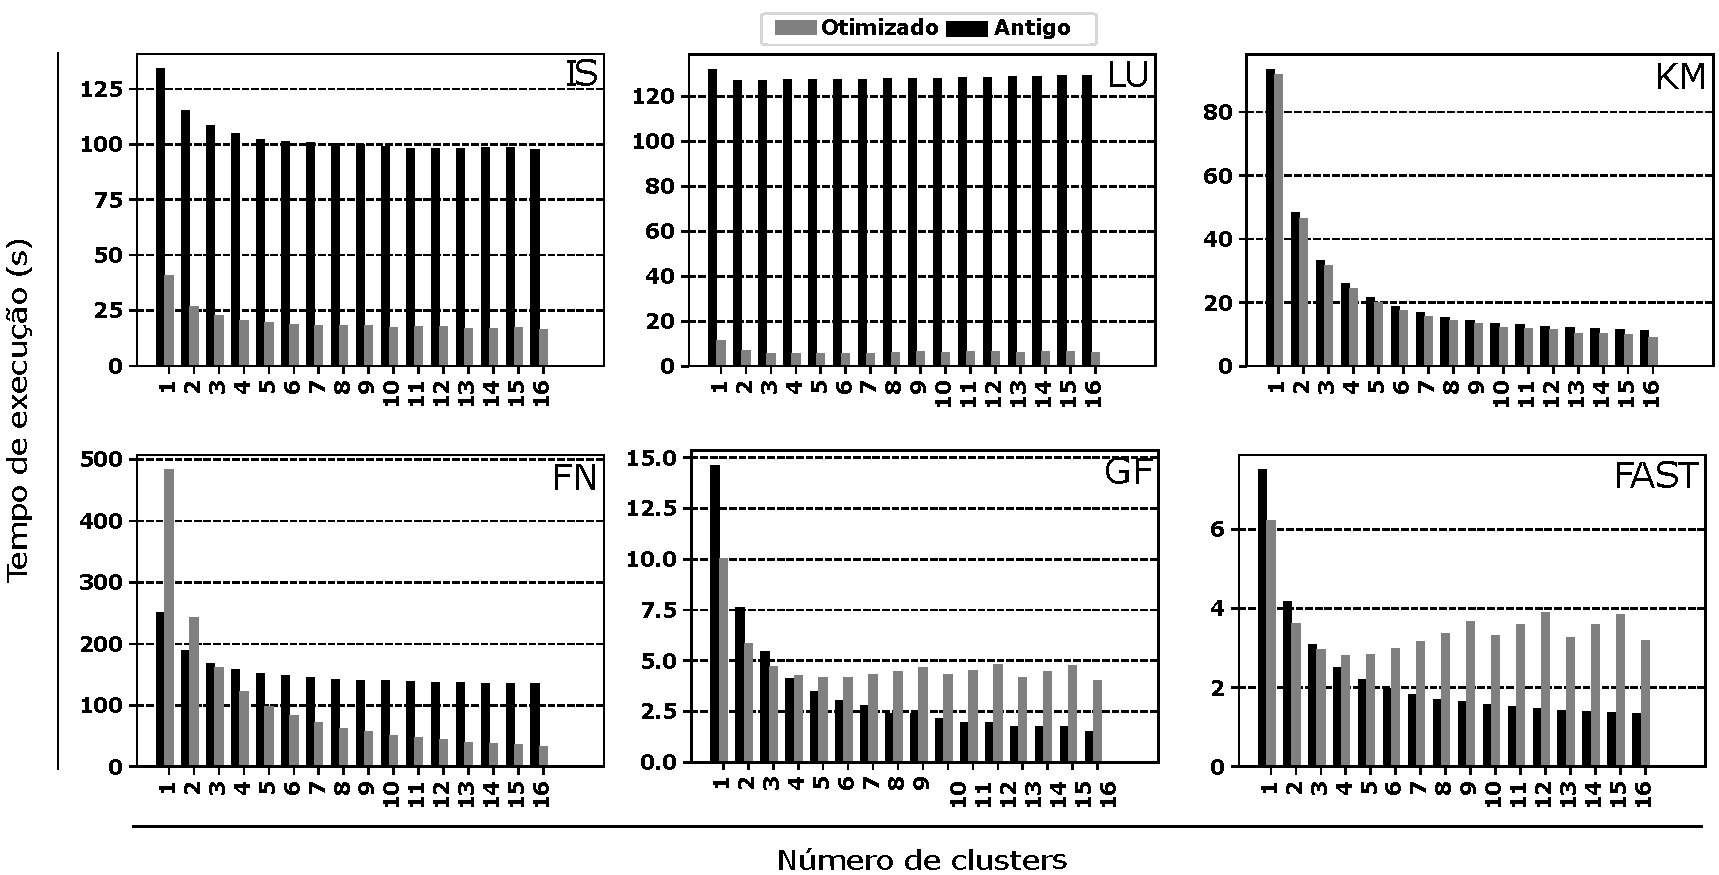
\includegraphics[width=15cm, keepaspectratio]{figs/execution-time.pdf}
\caption{Tempos de execução de cada aplicação, variando-se o número de \textit{clusters} para a classe \textit{default}.}\par
\label{fig:executiontime}
\end{figure}

\section{Resultados}
\label{sec:resultados}

Para coletar os resultados de desempenho das novas versões das aplicações, cada aplicação foi executada com a classe de problema \textit{default}, variando-se o número de \textit{clusters} no intervalo de 1 a 16. No \capb temos diversas classes de problemas, cada qual variando seu tamanho de entrada, podendo assim testar diferentes propriedades do \mppa. Cada variação foi repetida 10 vezes, obtendo-se o resultado final pela média das repetições, o qual observou-se desvio padrão menor que 1\%. Ademais, os resultados foram comparados com os obtidos por \textit{Souza} \etal \cite{Castro-Souza-CCPE:2016}. No geral, observa-se ganho em desempenho e, na média, redução de gasto energético também. 

O tempo de execução maior na versão antiga da FN, com uma pequena quantidade de \textit{clusters}, é esperado, já que toda lógica de comparação foi movida para os \ccs, utilizando assim mais núcleos de processamento, o que aumenta o número de comunicações e sincronizações entre \ccs (o que é parte da lógica). Da mesma maneira, como mais núcleos estão em execução, há aumento no consumo de energia. Porém, ao aumentar-se o número de \ccs, observa-se um ganho em desempenho. 

Também justifica-se o tempo e gasto energético maior nas aplicações GF e FAST. Os tempos mostrados nos gráficos consideram o tempo total de execução da aplicação (na nova versão excluímos o tempo de \textit{spawn} dos \textit{slaves}). Porém, as versões do \mppa em que cada versão do \capb rodou, antiga e nova, são diferentes, possuindo peculiaridades próprias que afetam no tempo de execução, quando este aproxima-se de 0, onde tais peculiaridades não são medidas diretamente dentro do \capb. Estas peculiaridades não tem relação com a \async e podem criar um viés de que o resultado piorou, quando isto não é verdade.

Ambas as aplicações, FAST e GF, estão com a mesma lógica, pois utilizam o \textit{master} somente para definição de tarefas e os \textit{slaves} para os cálculos. Assim, ao analisar os tempos médios de computação dos \textit{slaves} e de comunicação, vemos uma redução em todas as variações de execução, como por exemplo, na variação de execução com a classe \textit{default} utilizando 16 \textit{clusters}, onde o tempo médio dos \ccs foi de 0,8 segundos para a versão antiga, tomando 1,7 segundos de comunicação, enquanto que na nova, o tempo médio foi de 0,36 segundos, utilizando 1,08 segundos de comunicação. Da mesma maneira, como o gasto energético considera todo o tempo de execução, ou seja, o total citado acima, este também ficou maior para as aplicações GF, FAST e KM.

\begin{figure}[t]
\centering
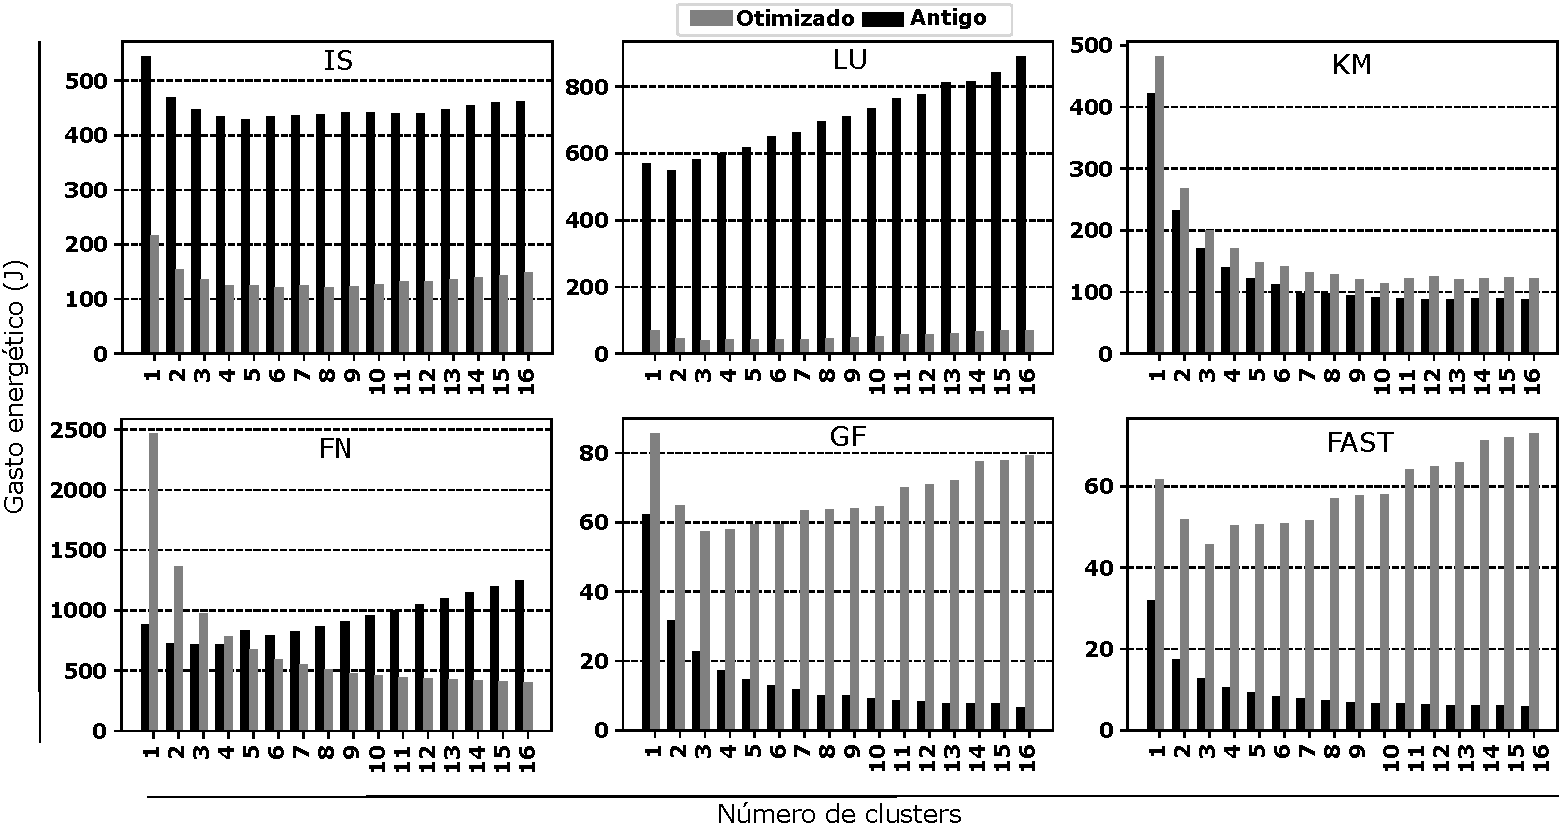
\includegraphics[width=15cm, keepaspectratio]{figs/power.pdf}
\caption{Gasto energético cada aplicação, variando-se o número de \textit{clusters} para a classe \textit{default}.}\par
\label{fig:executiontime}
\end{figure}

\section{Conclusão}
\label{sec:conclusao}

Neste trabalho, foram propostas otimizações para as aplicaçõe do \capb no \mppa, a fim de reduzir gasto energético e tempo de execução. Os resultados mostraram que houve esta redução para algumas das aplicações, através do uso da \async, mas para outras, considerando o tempo total, não. Como trabalhos futuros, pretende-se estudar a fundo as peculiaridades que afetam o tempo total, citadas na seção de resultados, a fim de poder medi-las e excluí-las do tempo total, quando necessário, para realizar uma comparação mais justa, focando nas \apis \async e \ipc. Além disso, pretende-se atualizar a implementação do \capb com a \api \ipc, de modo a torná-la equivalente a implementação utilizando a \async, podendo assim realizar uma comparação totalmente voltada para as \apis de comunicação.

\section{Avaliação PIBIC: Benefícios e Formação Científica}

Este projeto de pesquisa contribuiu de inúmeras formas para minha formação acadêmica. Do começo ao fim foi algo engrandecedor e acredito que, ao longo da minha carreira profissional, irei utilizar diversos conhecimentos aqui adquiridos. Este foi o primeiro projeto no qual tive contato com uma documentação de \api, e, assim como nosso primeiro contato com qualquer tecnologia nova, foi bastante desafiador. Através de muita dedicação e ajuda do meu orientador e colegas de trabalho, consegui quebrar as barreiras do conhecimento e entender a fundo como funciona a nova \api da Kalray, a \async.  

Neste ciclo de pesquisa também produzi um artigo científico, o qual foi aprovado na décima nona Escola Regional de Alto Desempenho da Região Sul (ERAD/RS 2019), ocorrida na cidade de Três de Maio, no Rio Grande do Sul. Com esta aprovação, fui apresentá-lo nesta mesma cidade na data de realização do evento. Participar deste evento foi também uma experiência enriquecedora, pois pude conhecer projetos de diferentes níveis de complexidade, englobando tanto projetos de iniciação cientifica quanto os do estado da arte.

Com este projeto de pesquisa pude também descobrir o que pretendo seguir na minha carreia profissional, assim como ter plena certeza de que de quero continuar com a pesquisa e contribuir de forma significativa para o avanço tecnológico de toda comunidade científica. Utilizarei também os resultados deste para realização do meu trabalho de conclusão de curso, onde pretendo expandir o que já foi pesquisado, realizando comparações com outros processadores do estado da arte.
 
\bibliography{bibliografia} 
\bibliographystyle{sbc}

\end{document}
